% !TEX root = main.tex
\chapter{Introduction}

  \begin{figure}
    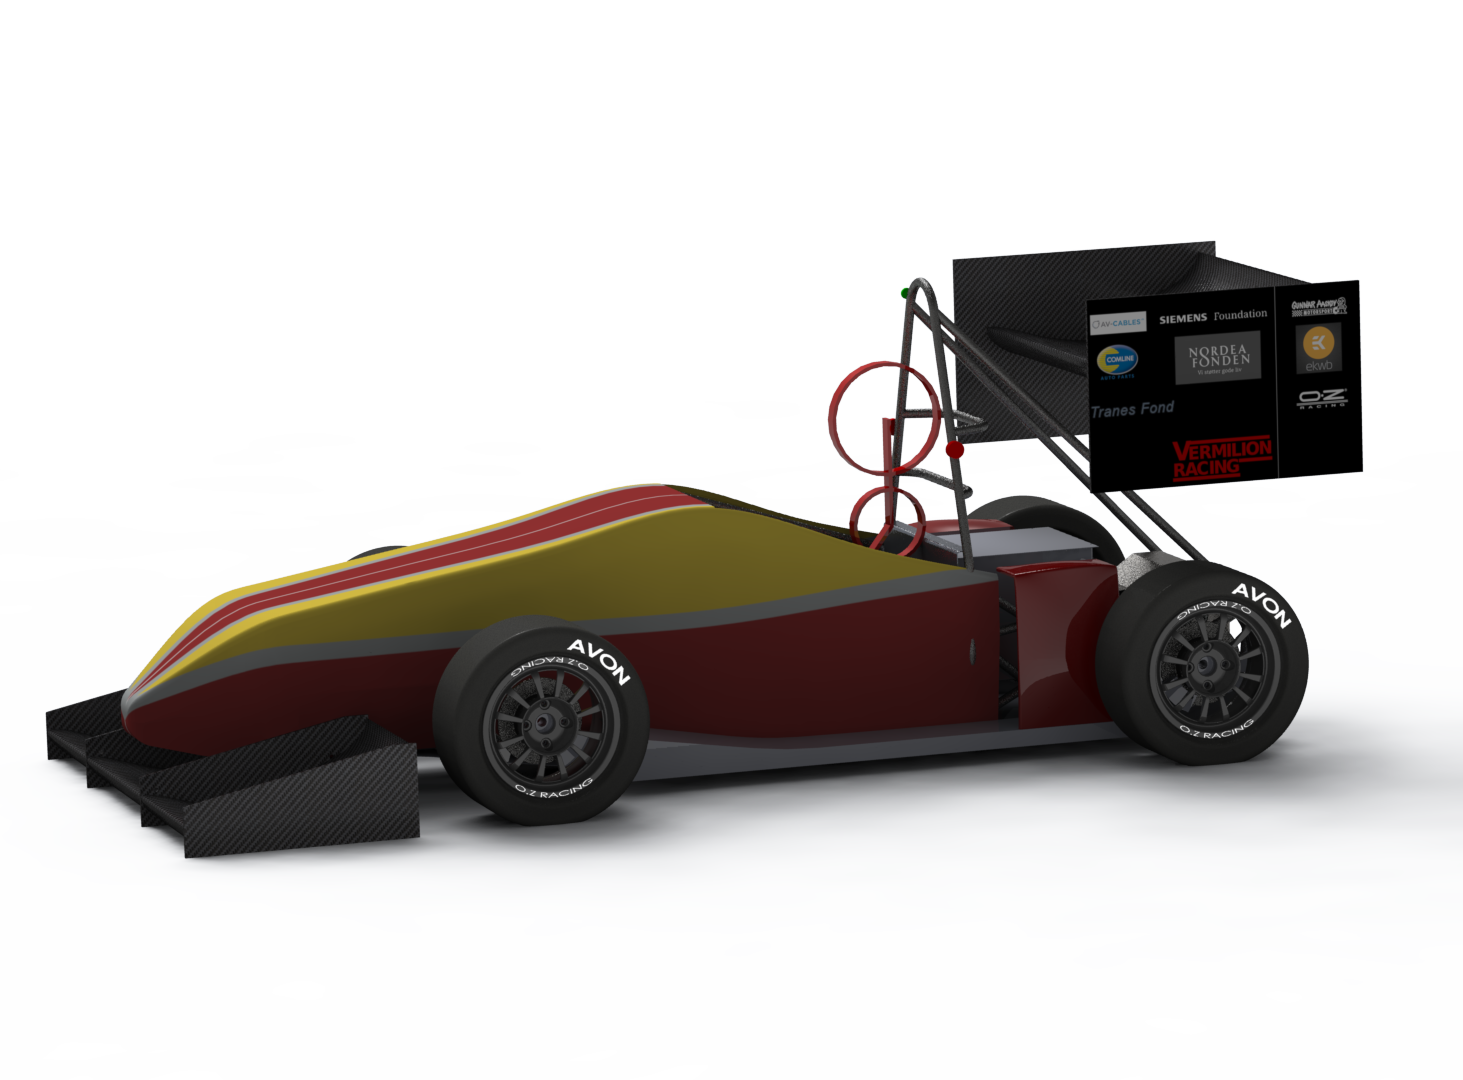
\includegraphics[width=\textwidth]{eveeRender_nobg}
    \caption{The teams' race car with the conceptual design of the rear wing.}
    \label{fig:EeveeRender}
  \end{figure}

  \textsc{Vermilion Racing} is a newly started electric race car team at DTU building their very first vehicle: The Eevee \cite{bulba}. The teams' purpose is to compete against other universities at the Silverstone race track from the 11\textsuperscript{th} to the 16\textsuperscript{th} of July. As members of the team, the purpose of this report is to document the design process of the rear wing of the first car, and provide the ground works towards a full aerodynamic package for future students on the team. A render of the car's design as of the 31\textsuperscript{st} of June is shown in figure \ref{fig:EeveeRender}. As this is the first car, this project sets out to uncover the requirements, theory and know-how behind building a rear wing.

  Aerodynamics is a major decider in racing today. Cornering, not top speed is the deciding factor amongst the teams, and aerodynamics is the key. Drag, lift and side force are the three cornerstones to vehicle aerodynamics. A car's ability to handle depends on the grip of the tyres, and downforce directly increases grip by increasing the downwards load on the tyres without adding a weight penalty. Additionally, drag directly decreases the speed of a vehicle by increasing air resistance, but is of less importance as the cars of this class have far more accelerative power than the tyres can handle \cite{jkatz}. Designing the bodyworks of Eevee is therefore a dance of downforce.

  This bachelor thesis attempts to lay down the ground work for designing, optimizing and manufacturing the car's rear wing. Our advisor, Jens Honore Walther, proposed simulating the wing geometry in order to both reduce financial cost and quicken the optimization process. The objective of the numerical simulations is ultimately to create an easily producable wing in a very short timespan, that produces ample amounts of negative lift for the time spent in production.

  As this is the first year the team is designing and building a car, time and money for production is sparse. To validate the simulated optimizations, a wind tunnel test is performed on a down-scaled wing using Flow Similarity theory. The measurements are compared with the results from a computational fluid dynamics simulation performed in \emph{Star-CCM+} to verify the preciseness of the simulations. Based on this, $x$- and $y$-distance between the multi-element wings and angle of attack is then optimized for maximum downforce. The multi-element wing is taken from theoretical abstraction to reality by designing a physical wing. The position, deflection and dimensions of the wing is thoroughly described by the rules of the Formula Student competition, guiding the final design process. In the final chapter, theories regarding strength of sandwich-structured composites and carbon fiber molding are explained, in order to describe the design decisions. Finally, the end result is discussed and possible improvements to the wing and mounting system are listed.

  Measurements and tests have been carried out at the DTU Wind laboratory's Red wind tunnel with assistance from co-supervisor Robert Flemming Mikkelsen on the 19\textsuperscript{th} and 20\textsuperscript{th} of June.

  The entire project is publicly available on \url{https://github.com/carlegroen/bachelor_project_racecar_aero}, where all work files, data, various notes and CAD drawings can be found. The Formula Student team at DTU: Vermilion Racing can be followed on \url{fb.com/FSDTU}.

\section{Design Philosophy}
  Designing a car with hundreds, if not thousands of different factors is incredibly difficult. Therefore, determining which factors are most important for the car's performance is very crucial to the teams' success. As the timespan of this project is short, time sets a limitation on the complexity of the wing's dimension. In addition, since this is the first of its kind, no design decisions can be based on prior experience. Finally, the finances for building the car are tight. This forces us to choose a low-cost solution where basing the design on literature and the experience of competing teams is the ideal choice.

  The requirements for the wing are, that it has to be as low weight as possible, in order to ensure optimum acceleration of the car. Thereto, drag has to be kept low, but the effect from drag is near negligible, which will be explained in section \ref{sec:topspeed}. Lastly, we have to maximize the downforce provided by the wing. For future iterations, ensuring that the center of pressure is kept as constant as possible is essential. If the frontwing, undertray and rear wing's downforce don't scale equally with speed, the center of pressure will move during acceleration. This will make the car's handling unpredictable, and potentially limit the driver's confidence in the car.

\section{Problem Statement}

  A new aerodynamically beneficial structure is to be implemented at the rear of the Eevee with the purpose of increasing the tyre's grip without adding a weight penalty. The goal is to have a cheap, both time- and money-wise, rear wing, which provides enough negative lift to benefit the car's lap time.
